%%%%%%%%%%%%%%%%%%%%%%%%%%%
% IEEE Submission Dashboard - https://ieee.atyponrex.com/submission/dashboard
%%%%%%%%%%%%%%%%%%%%%%%%%%%

% IEEE Transactions on human--machine systems
% https://ieeexplore.ieee.org/xpl/mostRecentIssue.jsp?punumber=6221037

%---------------------------------------------------------------------
% \documentclass[10pt,journal,compsoc]{IEEEtran}
% \documentclass[lettersize,journal]{IEEEtran}
% \documentclass[letterpaper,journal]{IEEEtran}
\documentclass[journal]{IEEEtran}
% ==== Core packages (normalized) ====

% How to hide statements:
%   - To enable  tags: \iftrue  and \fi
%   - To disable tags: \iffalse and \fi
% How to turn-on (or turn-off) page number:
%   - To turn-on  the page number: {plain}
%   - To turn-off the page number: {empty}
% Usage (Syntax):
%   \documentstyle[twocolumn]{article}
%   \pagestyle{empty}
%    ...
%   \maketitle
%   \thispagestyle{empty}

% How to print the page number at each page
\pagestyle{empty}

\usepackage[T1]{fontenc}
\usepackage[utf8]{inputenc}
\usepackage{microtype}
\usepackage{amsmath,amssymb}
\usepackage{amsthm}  % theorem 환경을 사용하기 위한 필수 패키지
%\usepackage{amsmath}
%\usepackage{amssymb}
\usepackage{makecell}
%\usepackage{amsmath,amsfonts,amssymb,mathtools}
%\usepackage{amsthm}
\usepackage{graphicx}
\usepackage{booktabs}
\usepackage{siunitx}
\usepackage{xspace}
\usepackage{pifont}
% Checkmark / Xmark symbols
\newcommand{\cmark}{\ding{51}}
\newcommand{\xmark}{\ding{55}}

\usepackage{listings}
\usepackage{xcolor}
\usepackage{xurl}
\usepackage{url}

% Hyperlinks to content
% \usepackage[linktocpage=true]{hyperref}
% \usepackage{hyperref}
% \usepackage[nameinlink]{cleveref}
% \usepackage[hidelinks]{hyperref}
\usepackage[colorlinks=true,linkcolor=blue,citecolor=blue,urlcolor=black]{hyperref}

\usepackage{cleveref}
%\usepackage{amsmath,amsfonts}
% \usepackage{algorithmic}
\usepackage{algorithm}
\usepackage{array}
\usepackage[caption=false,font=normalsize,labelfont=sf,textfont=sf]{subfig}
\usepackage{textcomp}
\usepackage{stfloats}
\usepackage{verbatim}
\usepackage{cite}
%\hyphenation{op-tical net-works semi-conduc-tor IEEE-Xplore}
%\usepackage{amssymb,amsmath,amsthm,mathtools}
%\usepackage{hyphenat}

%% ------------- ORC ID Template: Start ----------------------
% https://tex.stackexchange.com/questions/498688/orcid-in-latex-file-of-ieee-trans-in-a-customized-position

\usepackage{scalerel}
\usepackage{tikz}
\usetikzlibrary{svg.path,positioning,arrows.meta,shapes.geometric,calc}

\definecolor{orcidlogocol}{HTML}{A6CE39}
\tikzset{
orcidlogo/.pic={
\fill[orcidlogocol] svg{M256,128c0,70.7-57.3,128-128,128C57.3,256,0,198.7,0,128C0,57.3,57.3,0,128,0C198.7,0,256,57.3,256,128z};
\fill[white] svg{M86.3,186.2H70.9V79.1h15.4v48.4V186.2z}
svg{M108.9,79.1h41.6c39.6,0,57,28.3,57,53.6c0,27.5-21.5,53.6-56.8,53.6h-41.8V79.1z M124.3,172.4h24.5c34.9,0,42.9-26.5,42.9-39.7c0-21.5-13.7-39.7-43.7-39.7h-23.7V172.4z}
svg{M88.7,56.8c0,5.5-4.5,10.1-10.1,10.1c-5.6,0-10.1-4.6-10.1-10.1c0-5.6,4.5-10.1,10.1-10.1C84.2,46.7,88.7,51.3,88.7,56.8z};
}
}

\newcommand\orcidicon[1]{\href{https://orcid.org/#1}{\mbox{\scalerel*{

\begin{tikzpicture}[yscale=-1,transform shape]
    \pic{orcidlogo};
\end{tikzpicture}
}{|}}}}

%% ------------- ORC ID Template: End ----------------------

\providecommand{\cmark}{\ding{51}}
\providecommand{\xmark}{\ding{55}}
\providecommand{\etal}{\textit{et al.}\xspace}
\DeclareMathOperator{\E}{\mathbb{E}}
\DeclareMathOperator{\Var}{\mathrm{Var}}

\theoremstyle{plain}
\newtheorem{theorem}{Theorem}[section]
\newtheorem{lemma}{Lemma}[section]
\newtheorem{corollary}{Corollary}[section]
\lstdefinelanguage{json}{
basicstyle=\ttfamily\small,
numbers=left,
numberstyle=\tiny,
stepnumber=1,
showstringspaces=false,
breaklines=true
}
\lstset{frame=single}
% === End patch ===

\IEEEoverridecommandlockouts

%####################################################### Geunsik Area ###########

\usepackage{algorithm}
\usepackage{algpseudocode}

% LaTeX에서 유니코드(①, ② 등)를 직접 사용
\usepackage{pifont}

% theorem, algorithm 가독성위해 디자인 개선
\usepackage[most]{tcolorbox}
\tcbuselibrary{listings}

%% To keep strictly tuned whitespace rules among sections (e.g., section, subsection, and subsubsection)
%% for decreasing or increasing the vertical space between sections
\usepackage{titlesec}
\titlespacing*{\section}{0.70pt}{0.50\baselineskip}{0.20\baselineskip}
\titlespacing*{\subsection}{0.70pt}{0.50\baselineskip}{0.20\baselineskip}
\titlespacing*{\subsubsection}{0.70pt}{0.50\baselineskip}{0.20\baselineskip}

%% Reduce vertical space (padding) after figure (a big effect)
%% Warning: "Text page 7 contains only floats."
%% https://www.reddit.com/r/LaTeX/comments/b4mipa/how_to_decrease_space_between_paragraph_and/
\setlength{\textfloatsep}{0.70pt}
\setlength{\abovecaptionskip}{0.70pt}
\setlength{\belowcaptionskip}{0.70pt}

\theoremstyle{definition}
\newtheorem{definition}{Definition}[section]
\urlstyle{tt}

\newcommand{\Lninetyfive}{L_{95}}
\newcommand{\Jain}{\mathcal{J}}
\providecommand{\cmark}{\ding{51}}
\providecommand{\xmark}{\ding{55}}

% JSON language for listings
\lstdefinelanguage{json}{
basicstyle=\ttfamily\small,
numbers=left, numberstyle=\tiny, stepnumber=1,
showstringspaces=false,
breaklines=true
}

% Listings setup (handles code blocks and JSON/diff-like listings)
\lstset{basicstyle=\ttfamily\small, breaklines=true, columns=fullflexible, showstringspaces=false}

% Minimal JSON language for listings
\lstdefinelanguage{json}{
basicstyle=\ttfamily\small,
showstringspaces=false,
morestring=[b]",
morecomment=[l]{//},
literate=
*{0}{{{\color{black}0}}}{1}
{1}{{{\color{black}1}}}{1}
{2}{{{\color{black}2}}}{1}
{3}{{{\color{black}3}}}{1}
{4}{{{\color{black}4}}}{1}
{5}{{{\color{black}5}}}{1}
{6}{{{\color{black}6}}}{1}
{7}{{{\color{black}7}}}{1}
{8}{{{\color{black}8}}}{1}
{9}{{{\color{black}9}}}{1}
{:}{{{\color{black}{:}}}}{1}
{,}{{{\color{black}{,}}}}{1}
{"}{{{\color{black}{"}}}}{1}
}


\begin{document}

    %----------------------------------------\input{./001-title}

    \title{From Alerts to Actions: An Action-Centered Human--AI Decision Support Framework for Disaster Response}

    %---------------------------------- \input{./003-author}

    \author{

    % for ORC-ID
    \IEEEauthorblockN{
    Geunsik Lim$^{\textsuperscript{\orcidicon{0000-0003-1845-7132}}}$
    }


    \thanks{G. Lim is with the Department of Electrical and Computer Engineering, Sungkyunkwan University, 2066, Seobu-ro, Jangan-gu, Suwon 16419, South Korea (e-mail: leemgs@g.skku.edu). }

    }

    % The paper headers
    % \markboth{Journal of \LaTeX\ Class Files,~Vol.~14, No.~8, August~2015}%
    % {Shell \MakeLowercase{\textit{et al.}}: Bare Demo of IEEEtran.cls for IEEE Transactions on Magnetics Journals}

    \markboth{IEEE Transactions on Human-Machine Systems}{Lim: From Alerts to Actions: Action-Centered Human--AI Decision Support}

    % make the title area
    \maketitle

    \thispagestyle{empty}%

    % -----------------------------\input{./005-abstract}
    \begin{abstract}
        Human--AI decision systems are increasingly used where an inappropriate or delayed human action can have serious consequences, yet better AI predictions do not by themselves lead to appropriate human action. Drawing on the joint cognitive systems perspective, which evaluates the human and the machine as a single system, we present the \emph{Action-Centered Human--AI Decision Framework (ACHDF)}. ACHDF instantiates uncertainty-aware risk estimation, guardrailed AI recommendations, and human-in-the-loop escalation for disaster-response decision support, and it treats human action execution as the primary evaluation outcome. In a counterbalanced within-subjects study ($n=52$, 20 trials per participant), we compared an ACHDF-based prototype with a conventional dashboard in a simulated disaster-response task. The ACHDF condition was associated with a higher action execution rate (0.81 vs.\ 0.62; paired difference $+0.19$, 95\% CI [0.14, 0.25], $d_z = 0.96$), shorter response latency (8.1 vs.\ 12.4~s), lower self-reported workload (NASA--TLX), and higher perceived trust and usability (all $p < .001$; Holm-adjusted for the secondary outcomes). All failed trials were wrong selections, wrong and correct trials had the same latency, and no order or carry-over effect was detected. Because the two conditions differed in several features at once, the results describe the integrated ACHDF configuration rather than individual components, and the study cannot assess trust calibration or automation bias. Validation in other domains and with professional operators remains future work.
    \end{abstract}

    \begin{IEEEkeywords}
        Human--AI decision systems, joint cognitive systems, adaptive automation, human-in-the-loop, trust in automation, cognitive workload, action execution
    \end{IEEEkeywords}

    %--------------------------------------- \input{./010-introduction}
\section{Introduction}
\IEEEPARstart{H}{uman}--AI decision systems are increasingly used in situations with high uncertainty, high stakes, and severe time pressure \cite{Bach2024Access,PerezCerrolaza2024CSUR,Yang2022THMSReview}, for example in healthcare triage, supervision of autonomous vehicles, industrial safety, and emergency response \cite{Rokhideh2025IJDRS,Rao2024IJDRS,lim2026generativeaidrivenreliabilitylayer}. AI is mainly used there to improve prediction, but human--machine systems research has repeatedly shown that better predictions do not necessarily lead to appropriate human action \cite{Lai2023FAccT,Muller2022CHIWORK,Hodgson2013THMS}.

AI outputs are typically shown as probabilities or alarms, often communicating uncertainty poorly or only implicitly, with little support for turning them into action \cite{Weidinger2022FAccT,Miller2019XRDS,Bach2024Access}. The human is left to close the loop between prediction and action, often under cognitive stress \cite{Hodgson2013THMS,Zhang2022THMS}. Operators may wait for confirmation, disregard advice they do not trust, or over-rely on an AI whose accuracy is overstated \cite{Hodgson2013THMS,Raji2019AIES,Raji2022CACM,Parasuraman2010}. Without explicit support for appropriate trust, workload management, and human override, decision support can increase automation bias or workload and lose its intended benefit \cite{Zhang2022THMS,Bach2024Access,Lee2004}.

These concerns are not new to cognitive systems engineering. The joint cognitive systems (JCS) perspective holds that a human and a machine working together form a single cognitive system that should be evaluated by the outcomes it jointly produces, not by the performance of the machine alone \cite{Hollnagel2005JCS,Woods2006JCS}. Research on adaptive automation and levels of automation has likewise studied how support should change with task demands while keeping the human in control \cite{Parasuraman2000LOA,Kaber2004,Scerbo2007}. Much current work on AI-based decision support, however, still evaluates systems by prediction accuracy or usability rather than by whether the human--AI system produces appropriate and timely action \cite{Lai2023FAccT,Muller2022CHIWORK,Yang2022THMSReview,lim2026generativeaidrivenreliabilitylayer}. This paper applies the JCS perspective to AI-assisted disaster-response decision support and tests it empirically.

We address the following, deliberately scoped research question:
\begin{quote}
    \emph{Compared with a conventional dashboard, is an ACHDF-based decision support system associated with better action execution in a simulated, high-uncertainty disaster-response task, and how does it relate to response latency, workload, and trust?}
\end{quote}
The study examined four hypotheses: \textbf{H1 (primary)}, the Action Execution Rate (AER) is higher in the AI-assisted (ACHDF) condition than in the baseline; and, as secondary hypotheses, \textbf{H2} response latency is shorter, \textbf{H3} self-reported workload (NASA--TLX) is lower, and \textbf{H4} perceived trust and usability are higher in the AI-assisted condition. Action execution is thus the primary outcome, and latency, workload, trust, and usability are secondary outcomes. Trust and workload also act as \emph{design considerations} that shaped how information is presented, but the implemented system does not measure or adapt to them at run time (Section~\ref{sec:constructs}).

The contributions of this paper are as follows. First, we apply the JCS principle of evaluating joint human--machine outcomes to AI-assisted disaster decision support, with action execution as the primary evaluation outcome; the principle is established \cite{Hollnagel2005JCS,Woods2006JCS}, and our contribution is to make it concrete for an area where AI systems are usually evaluated by accuracy alone. Second, we present ACHDF, a domain-specific instantiation of the JCS and adaptive function allocation perspectives that combines uncertainty-aware risk estimation, guardrailed recommendations, and uncertainty- and criticality-triggered escalation, while the human keeps final decision authority. Third, we report a controlled within-subjects evaluation ($n=52$) comparing the integrated ACHDF configuration with a conventional dashboard on action execution, latency, workload, trust, and usability. Because several features differed between conditions, it does not isolate individual ACHDF components.


    %----------------------------- \input{./020-related_work}
\section{Related Work}
This section reviews the streams of work that ACHDF builds on: joint cognitive systems and adaptive function allocation, which form its conceptual basis; decision support, trust, workload, and automation bias; and AI assistance in high-stakes environments.

\subsection{Joint Cognitive Systems and Adaptive Function Allocation}
Cognitive systems engineering treats a human operator and the technology the operator works with as a \emph{joint cognitive system} (JCS); the unit of analysis is the joint system and the outcomes it produces in its work environment, not the machine's internal performance \cite{Hollnagel2005JCS,Woods2006JCS}. Evaluating decision support by the actions the joint system executes is therefore a natural consequence of this stance, not a new concept, and ACHDF adopts it explicitly.

A second body of work addresses how functions are allocated between humans and automation. Parasuraman \emph{et al.} distinguish types of automation (information acquisition, information analysis, decision selection, and action implementation) and levels of automation within each \cite{Parasuraman2000LOA}. Adaptive automation changes the level or type of support in response to task demands, operator state, or critical events \cite{Scerbo2007,Kaber2004}; higher levels of decision support can reduce situation awareness and leave operators unprepared when automation fails \cite{Kaber2004,Parasuraman2010}.

ACHDF relates to this literature in three ways. (i) In the terms of Parasuraman \emph{et al.} \cite{Parasuraman2000LOA}, it automates information analysis and decision selection (risk estimation and recommendation) but never action implementation: the human always executes the action. (ii) Its adaptation is \emph{event-triggered}: the form of support changes when estimated uncertainty, action criticality, or a policy check crosses a threshold (Algorithm~\ref{alg:escalation}), not in response to measured operator workload or physiological state. (iii) What changes is the \emph{level and form of AI support}, from a bounded recommendation to an escalated presentation of evidence and options; decision authority does not move between AI and human. ACHDF therefore proposes no new allocation theory but a domain-specific instantiation of these principles for AI-generated recommendations in disaster response.

\subsection{Decision Support, Trust, Workload, and Automation Bias}
Systems that only display predictions leave interpretation and decision making to the user, which is costly under time pressure \cite{Bach2024Access,PerezCerrolaza2024CSUR}, and what matters is also how recommendations enter the human decision process \cite{Lai2023FAccT,Muller2022CHIWORK,Hodgson2013THMS}. This has motivated decision support that offers actionable recommendations while keeping the human in control and responsible \cite{Assaad2023TAS,Yang2022THMSReview}.

Trust in automation is commonly defined as the attitude that an agent will help achieve an individual's goals in a situation characterized by uncertainty and vulnerability; \emph{appropriate} (calibrated) trust means that reliance matches the automation's actual capabilities \cite{Lee2004}. Over-trust can lead to misuse and automation bias, in which automation errors go undetected, and under-trust to disuse \cite{Lee2004,Parasuraman2010,Raji2019AIES,Raji2022CACM}. Automation bias is most likely when automation is highly but not perfectly reliable and its uncertainty is not represented \cite{Parasuraman2010,Weidinger2022FAccT}. Assessing calibration directly requires comparing reliance with the correctness of the advice, including trials in which it is wrong \cite{Lee2004,Parasuraman2010}. Workload is commonly measured with the NASA Task Load Index (NASA--TLX) \cite{Hart1988}.

\subsection{AI Assistance in High-Stakes Environments}
AI-assisted decision systems are increasingly used for time-critical decisions in healthcare, aviation, and emergency management \cite{PerezCerrolaza2024CSUR,Bach2024Access,Rokhideh2025IJDRS,Rao2024IJDRS}, yet higher predictive accuracy does not guarantee better human performance \cite{Lai2023FAccT,Yang2022THMSReview}. Work on responsible and explainable AI stresses human-in-the-loop controls \cite{Weidinger2022FAccT,Assaad2023TAS,Miller2019XRDS,PerezCerrolaza2024CSUR} but is mostly conceptual or algorithm-centric, and few studies have examined empirically how design features such as uncertainty-aware escalation and guardrails affect the actions humans take \cite{Bach2024Access,Lai2023FAccT}. In disaster response, the input to the risk layer of ACHDF (Section~\ref{sec:system}) comes from heterogeneous sensor networks, ad hoc communications, and community reporting \cite{Yang2005MobiHoc,Longo2025PMC}. How such upstream information is fused is outside the scope of this paper.


%-----------------------------input{./050-design}



    \begin{figure}[t]
        \centering
        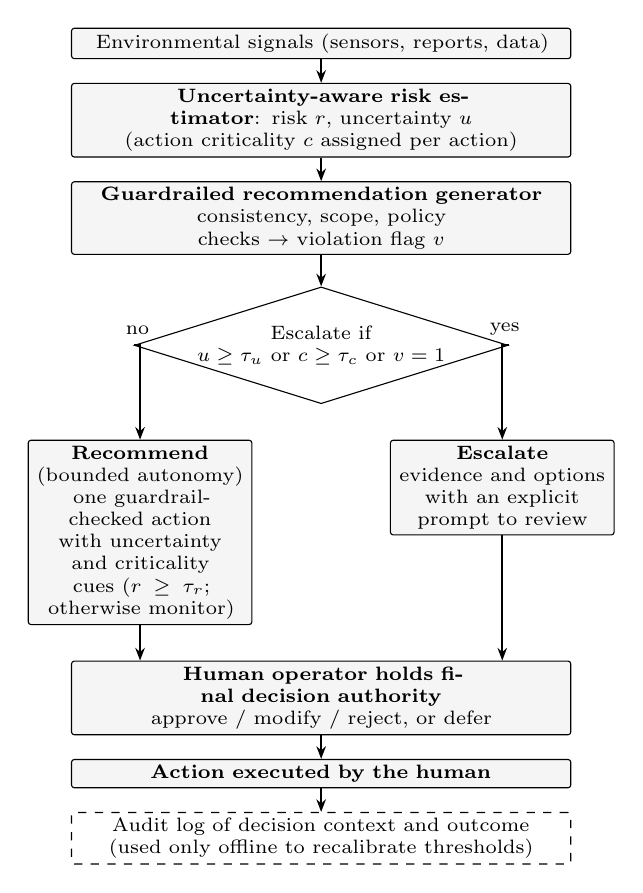
\begin{tikzpicture}[
            font=\scriptsize, node distance=3mm,
            box/.style={draw, rounded corners=1pt, align=center, fill=gray!8, text width=#1, inner sep=2pt},
            box/.default=6.2cm,
            dec/.style={draw, diamond, aspect=3.2, align=center, fill=white, inner sep=0pt},
            arr/.style={-{Stealth[length=1.6mm]}, thick}]
            \node[box] (env) {Environmental signals (sensors, reports, data)};
            \node[box, below=of env] (risk) {\textbf{Uncertainty-aware risk estimator}: risk $r$, uncertainty $u$\\(action criticality $c$ assigned per action)};
            \node[box, below=of risk] (gen) {\textbf{Guardrailed recommendation generator}\\consistency, scope, policy checks $\rightarrow$ violation flag $v$};
            \node[dec, below=4mm of gen] (pol) {Escalate if\\$u \ge \tau_u$ or $c \ge \tau_c$ or $v = 1$};
            \node[box=2.7cm, anchor=north] (rec) at ($(pol.south)+(-2.3,-0.45)$) {\textbf{Recommend} (bounded autonomy)\\one guardrail-checked action with uncertainty and criticality cues ($r \ge \tau_r$; otherwise monitor)};
            \node[box=2.7cm, anchor=north] (esc) at ($(pol.south)+(2.3,-0.45)$) {\textbf{Escalate}\\evidence and options with an explicit prompt to review};
            \node[box, anchor=north] (hum) at ($(rec.south -| pol.south)+(0,-0.45)$) {\textbf{Human operator holds final decision authority}\\approve / modify / reject, or defer};
            \node[box, below=of hum] (act) {\textbf{Action executed by the human}};
            \node[box, below=of act, fill=white, dashed] (log) {Audit log of decision context and outcome\\(used only offline to recalibrate thresholds)};
            \draw[arr] (env) -- (risk); \draw[arr] (risk) -- (gen); \draw[arr] (gen) -- (pol);
            \draw[arr] (pol.west) -| node[above, pos=0.3] {no} (rec.north);
            \draw[arr] (pol.east) -| node[above, pos=0.3] {yes} (esc.north);
            \draw[arr] (rec.south) -- (rec.south |- hum.north);
            \draw[arr] (esc.south) -- (esc.south |- hum.north);
            \draw[arr] (hum) -- (act); \draw[arr] (act) -- (log);
        \end{tikzpicture}
        \caption{Operational workflow of the proposed human--AI decision system.
The escalation test follows Algorithm~\ref{alg:escalation}. Depending on the estimated uncertainty, the action criticality, and the guardrail policy checks, the system either presents a bounded recommendation or escalates the case for human review with evidence and options (when $r < \tau_r$ and no trigger fires, the system only monitors). In both modes, the human operator holds final decision and execution authority. Trust and workload are not adapted at run time. The audit log is used only offline.}
        \label{fig:system_overview}
    \end{figure}

    \section{System Overview and Architecture}
    \label{sec:system}
    This section introduces the proposed human--AI decision system. The system is non-autonomous and human-centric: the AI analyzes information and proposes options, and the human decides and acts. The architecture follows the \textbf{Action-Centered Human--AI Decision Framework (ACHDF)}, which, following the joint cognitive systems perspective \cite{Hollnagel2005JCS,Woods2006JCS}, treats the human operator and the AI as one decision system whose goal is appropriate human action.

    ACHDF has four design layers: the \emph{environment and uncertainty context} (incomplete, time-pressured, asymmetric-risk conditions), \emph{uncertainty-aware risk modeling} (probabilistic risk estimates with explicit uncertainty), \emph{guardrailed AI decision support} (constrained, policy-aligned options), and \emph{human authority and accountability} (oversight, override, and responsibility). Two cross-cutting elements, appropriate trust \cite{Lee2004} and cognitive ergonomics, are design considerations (Table~\ref{tab:constructs}): they determined which cues are shown (e.g., explicit uncertainty indicators) and how much information is shown at once, but the implemented system neither measures nor adapts to them at run time.

    Fig.~\ref{fig:system_overview} depicts the run-time behavior. When model uncertainty is low and the action is not critical, the system presents a tightly scoped, action-oriented recommendation. We call this mode \emph{bounded autonomy}: the term refers only to the AI's freedom in \emph{generating} a recommendation, which is bounded by guardrails, and does not mean that the AI executes actions or holds decision authority. When uncertainty, criticality, or a policy check exceeds its threshold, the system switches to \emph{escalation}: instead of a single recommendation it presents the evidence and available options and explicitly asks the operator to review them. What varies between the two modes is thus the \emph{level and form of AI support}; final decision and execution authority stays with the human in both.

    \subsection{Constructs and Their Roles}
    \label{sec:constructs}
    Table~\ref{tab:constructs} summarizes the role of each ACHDF construct, i.e., whether it is a design input, a system state, a design consideration, or an evaluation outcome, together with its operational definition in the implemented system.

\begin{table*}[t]
\centering
\caption{ACHDF Constructs: Role, Operational Definition, and Implementation}
\label{tab:constructs}
\begin{tabular}{p{2.4cm} p{3.4cm} p{10.6cm}}
\toprule
\textbf{Construct} & \textbf{Role in ACHDF} & \textbf{Operational definition / implementation} \\
\midrule
Uncertainty $u$ & Design input; determines system mode & Dispersion of the posterior risk estimate (Section~\ref{sec:risk}); compared with threshold $\tau_u$. \\
Criticality $c$ & Design input; determines system mode & Severity of the consequences if the recommended action is wrong or delayed (cost of error); compared with threshold $\tau_c$. \\
Guardrails & Constraint on recommendation generation & Rule-based checks on every recommendation (Section~\ref{sec:guardrails}). In the framework, a failed check withholds the recommendation and escalates the case ($v=1$ in Algorithm~\ref{alg:escalation}); in the study prototype, a deny-list hit redacts the text instead. \\
Bounded autonomy & System mode (``recommend'') & The AI presents one scoped, guardrail-checked recommendation. The AI never executes actions; the human decides and acts. \\
Escalation & System mode (``escalate'') & Triggered if $u \ge \tau_u$, $c \ge \tau_c$, or a policy check fails ($v=1$). The system presents evidence and options and asks the operator to approve, modify, or reject. \\
Trust & Design consideration; secondary outcome & Shaped interface design (explicit uncertainty and criticality cues). Measured post-condition by questionnaire (Section~\ref{sec:measures}). Not adapted at run time. \\
Workload & Design consideration; secondary outcome & Shaped interface design (single consolidated view, action-oriented phrasing). Measured post-condition by NASA--TLX \cite{Hart1988}. Not adapted at run time. \\
Action execution & Primary outcome & Measured by AER (Section~\ref{sec:measures}). \\
\bottomrule
\end{tabular}
\end{table*}

    \subsection{Design Goals}
    Three goals follow from ACHDF. \textbf{Goal 1:} enable human \emph{action execution}, not only situational awareness and prediction accuracy. \textbf{Goal 2:} support appropriate trust \cite{Lee2004} by making uncertainty explicit, so that users can judge when to rely on the system and when on their own judgment. \textbf{Goal 3:} preserve human authority: operators always hold final decision-making and execution authority. In the terms of Parasuraman \emph{et al.} \cite{Parasuraman2000LOA}, the system automates information analysis and decision selection but not action implementation, and the level and form of support adapt to the estimated uncertainty and the criticality of the action.

    \subsection{Probabilistic Risk Estimation With Uncertainty}
    \label{sec:risk}
    Rather than a point estimate, the risk module outputs a posterior risk distribution, from which the risk level $r$ and the uncertainty $u$ are derived; together they determine whether the system presents a bounded recommendation or escalates (Algorithm~\ref{alg:escalation}). Explicit uncertainty is intended to avoid conveying false precision. This paper focuses on how the estimate and its uncertainty are used in the human--AI interaction, not on the risk model itself, whose estimation and calibration are not evaluated here (Section~\ref{sec:lim_reporting}).

    \textbf{Study prototype configuration.} The prototype used the configuration of the open reference implementation distributed with the paper (confirmed by the author): a Bayesian linear regression with a Gaussian prior on four normalized factors (hazard, exposure, vulnerability entered as $1-$vulnerability, and a social factor) plus an intercept (noise variance $\sigma^2=0.10$, prior variance $\tau^2=2.0$). The risk level $r$ is the posterior mean prediction clipped to $[0,1]$, and $u$ is the posterior variance. Two thresholds on $r$ yield an ``IMMEDIATE'' ($r \ge 0.8$), ``PREPARE'' ($0.6 \le r < 0.8$), or ``STAY ALERT'' ($r < 0.6$) message; a further configured value (0.3) is unused. These three levels are coarser than the five response options of the task (Section~\ref{sec:task}) and do not map one-to-one onto them. The configuration specifies no values for $\tau_u$ and $\tau_c$ and contains no code for the escalation branch of Algorithm~\ref{alg:escalation}: the algorithm is the framework specification, and in the study the escalation flag was pre-assigned per trial in the scenario design and logged.

    \subsection{Guardrailed AI Recommendation Module}
    \label{sec:guardrails}
    The recommendation module converts the risk estimate into a recommended action with a short justification. In the prototype, the text comes from three fixed message templates selected by risk band, so the output is template-based, not free-form generation. In the framework, every recommendation passes three guardrail checks before it is shown: (i) a \emph{consistency check}, so that the action does not contradict the risk estimate; (ii) a \emph{scope check}, so that the action comes from the set of permitted actions for the scenario; and (iii) a \emph{policy check}, for compliance with operational and safety rules. A recommendation that fails any check is withheld and the case is escalated ($v=1$).

    \textbf{Implementation in the study prototype.} Because the message is selected deterministically from $r$, it cannot contradict the risk estimate and is always a permitted message. The policy check is a deny-list filter (terms such as ``medical diagnosis'' and ``evacuation by force'' are replaced by ``[REDACTED]'', case-insensitively) plus expansion of technical terms into plain language. In the prototype, a policy hit therefore redacts text instead of triggering escalation; routing $v=1$ to escalation is part of the framework specification only. The criticality scale and its threshold $\tau_c$ are not documented. Each recommendation is displayed with criticality and confidence cues.
    \begin{algorithm}[t]
        \caption{Uncertainty-aware escalation and human override policy}
        \label{alg:escalation}
        \begin{algorithmic}[1]
            \Require risk estimate $r$, uncertainty $u$, action criticality $c$
            \Require policy-violation flag $v \in \{0,1\}$ from guardrail checks
            \Require thresholds $\tau_r, \tau_u, \tau_c$
            \If{$u \ge \tau_u$ \textbf{or} $c \ge \tau_c$ \textbf{or} $v = 1$}
            \State $\textsc{mode} \leftarrow \text{``escalate''}$ \Comment{route to human review}
            \ElsIf{$r \ge \tau_r$}
            \State $\textsc{mode} \leftarrow \text{``recommend''}$ \Comment{bounded autonomy}
            \Else
            \State $\textsc{mode} \leftarrow \text{``monitor''}$
            \EndIf
            \If{$\textsc{mode} = \text{``escalate''}$}
            \State Present evidence and options to operator
            \State Operator selects: approve / modify / reject / defer
            \ElsIf{$\textsc{mode} = \text{``recommend''}$}
            \State Present guardrail-checked recommendation
            \State Operator decides and executes, overrides, or defers
            \EndIf
            \State Log decision context and outcome for audit and calibration
        \end{algorithmic}
    \end{algorithm}

\subsection{Human Override and Escalation Mechanisms}
Escalation follows Algorithm~\ref{alg:escalation}: a case is escalated if uncertainty exceeds $\tau_u$, criticality exceeds $\tau_c$, or a guardrail check fails ($v=1$). Escalation is not a failure mode but a deliberate change in the form of support that keeps the operator accountable. In every mode, operators can accept, modify, or reject the AI's recommendation, and all operations are logged. This adaptation of the level of support follows established principles of adaptive automation \cite{Parasuraman2000LOA,Scerbo2007} and does not transfer decision authority to the AI.


    % -------------------------------\input{./060-evaluation}
    \section{Experimental Design and Methods}

    This section describes the controlled user study that compared the ACHDF-based system with a conventional dashboard; it is the only empirical evaluation reported. All statistics were recomputed from the anonymized trial-level logs (1,040 trials) and questionnaire records, and the data and analysis scripts are provided with the paper (Section~\ref{sec:data}). Details that remain undocumented are listed in Section~\ref{sec:lim_reporting}.

    \subsection{Study Design and Conditions}

    We used a within-subjects design with a \emph{baseline} and an \emph{AI-assisted} (ACHDF) condition in counterbalanced order (28 participants completed the AI-assisted condition first, 24 the baseline first). Both conditions were designed to present comparable scenario sets. Counterbalancing does not remove carry-over, since participants may have remembered scenarios from the first condition, so we tested order and carry-over effects (Section~\ref{sec:res_order}).

    \textbf{Baseline condition.} Participants used a conventional dashboard-style interface (Fig.~\ref{fig:interfaces}a): a risk-level summary (numeric value and color coding), a map or time series of risk indicators, and the five response-option buttons. It provided no AI-generated recommendation, uncertainty indicator, criticality cue, or escalation prompt, so participants had to integrate the information themselves.

    \textbf{AI-assisted condition.} The ACHDF-based interface displayed the same underlying information plus the ACHDF features of Section~\ref{sec:system}: a risk estimate with an uncertainty indicator (a confidence interval or variance proxy), a criticality badge, and either a single guardrail-checked recommendation with a short rationale (``recommend'' mode, e.g., ``PREPARE: Pack essentials, confirm route to shelter, check on neighbors.'') or, when escalation was triggered, the evidence and options with a message that human review was required because of uncertainty, criticality, or a policy issue (``escalate'' mode). The five response options remained selectable in both modes, so participants could ignore the recommendation, and both interfaces supported a deferral flag. Table~\ref{tab:conditions} and Fig.~\ref{fig:interfaces} contrast the two interfaces; the decision logic is in Fig.~\ref{fig:system_overview} and Algorithm~\ref{alg:escalation}. Fig.~\ref{fig:interfaces} is a reconstructed illustration drawn from the interface specification, not a screenshot; no screenshots of the study interface are available (Section~\ref{sec:lim_reporting}).

    \begin{figure*}[t]
        \centering
        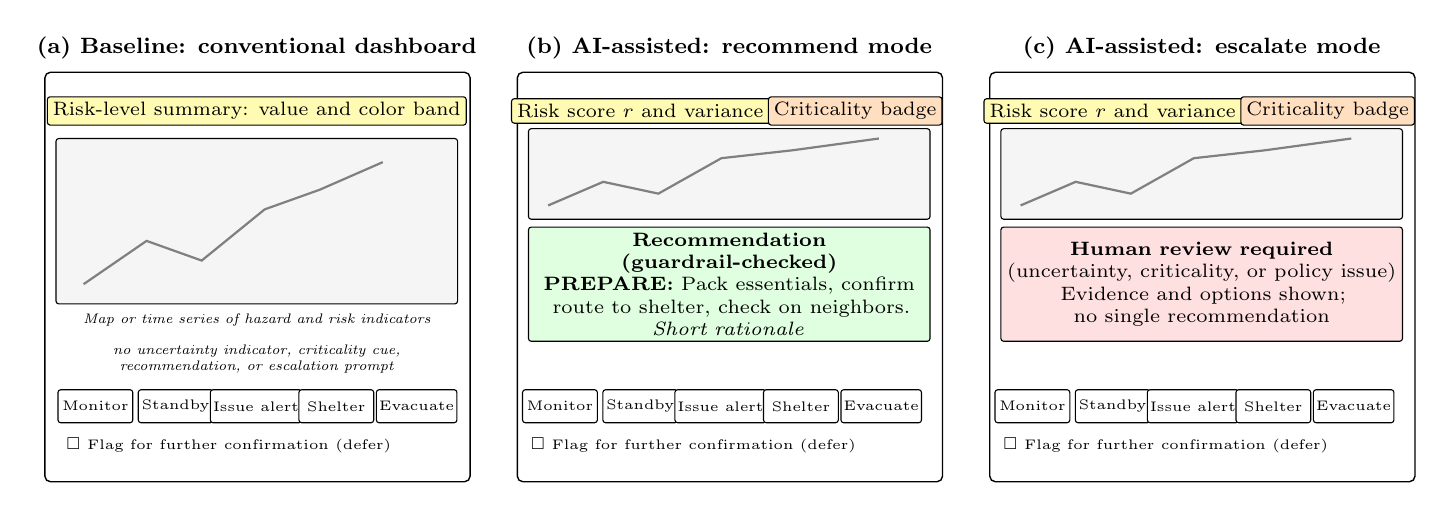
\begin{tikzpicture}[font=\scriptsize,
            frame/.style={draw, rounded corners=2pt, line width=0.5pt, fill=white},
            blk/.style={draw, rounded corners=1pt, align=center, inner sep=2pt, fill=gray!8},
            btn/.style={draw, rounded corners=1pt, align=center, inner sep=1pt, minimum height=0.42cm, fill=white, font=\tiny},
            ttl/.style={font=\footnotesize\bfseries}]
        % ---------- helper: five option buttons + defer flag, drawn at given x-offset and y
        \newcommand{\optionrow}[2]{%
          \node[btn, minimum width=0.95cm] at (#1+0.55,#2) {Monitor};
          \node[btn, minimum width=0.95cm] at (#1+1.57,#2) {Standby};
          \node[btn, minimum width=0.95cm] at (#1+2.59,#2) {Issue alert};
          \node[btn, minimum width=0.95cm] at (#1+3.61,#2) {Shelter};
          \node[btn, minimum width=0.95cm] at (#1+4.63,#2) {Evacuate};
          \node[anchor=west, font=\tiny] at (#1+0.05,#2-0.5) {$\square$ Flag for further confirmation (defer)};}
        % ---------- (a) baseline
        \node[ttl] at (2.6,0.45) {(a) Baseline: conventional dashboard};
        \node[frame, minimum width=5.4cm, minimum height=5.2cm, anchor=north west] (fa) at (-0.1,0.15) {};
        \node[blk, fill=yellow!30, minimum width=5.1cm] at (2.6,-0.35) {Risk-level summary: value and color band};
        \node[blk, minimum width=5.1cm, minimum height=2.1cm] at (2.6,-1.75) {};
        \draw[gray, thick] (0.4,-2.55) -- (1.2,-2.0) -- (1.9,-2.25) -- (2.7,-1.6) -- (3.4,-1.35) -- (4.2,-1.0);
        \node[font=\tiny\itshape] at (2.6,-3.0) {Map or time series of hazard and risk indicators};
        \node[font=\tiny\itshape, align=center] at (2.6,-3.5) {no uncertainty indicator, criticality cue,\\recommendation, or escalation prompt};
        \optionrow{-0.0}{-4.1}
        % ---------- (b) AI recommend
        \node[ttl] at (8.6,0.45) {(b) AI-assisted: recommend mode};
        \node[frame, minimum width=5.4cm, minimum height=5.2cm, anchor=north west] at (5.9,0.15) {};
        \node[blk, fill=yellow!30, minimum width=3.2cm] at (7.6,-0.35) {Risk score $r$ and variance $u$};
        \node[blk, fill=orange!25, minimum width=1.7cm] at (10.2,-0.35) {Criticality badge};
        \node[blk, minimum width=5.1cm, minimum height=1.15cm] at (8.6,-1.15) {};
        \draw[gray, thick] (6.3,-1.55) -- (7.0,-1.25) -- (7.7,-1.4) -- (8.5,-0.95) -- (9.4,-0.85) -- (10.5,-0.7);
        \node[blk, fill=green!12, minimum width=5.1cm, text width=4.9cm, minimum height=1.45cm] at (8.6,-2.55) {\textbf{Recommendation (guardrail-checked)}\\ \textbf{PREPARE:} Pack essentials, confirm route to shelter, check on neighbors.\\ \emph{Short rationale}};
        \optionrow{5.9}{-4.1}
        % ---------- (c) AI escalate
        \node[ttl] at (14.6,0.45) {(c) AI-assisted: escalate mode};
        \node[frame, minimum width=5.4cm, minimum height=5.2cm, anchor=north west] at (11.9,0.15) {};
        \node[blk, fill=yellow!30, minimum width=3.2cm] at (13.6,-0.35) {Risk score $r$ and variance $u$};
        \node[blk, fill=orange!25, minimum width=1.7cm] at (16.2,-0.35) {Criticality badge};
        \node[blk, minimum width=5.1cm, minimum height=1.15cm] at (14.6,-1.15) {};
        \draw[gray, thick] (12.3,-1.55) -- (13.0,-1.25) -- (13.7,-1.4) -- (14.5,-0.95) -- (15.4,-0.85) -- (16.5,-0.7);
        \node[blk, fill=red!12, minimum width=5.1cm, text width=4.9cm, minimum height=1.45cm] at (14.6,-2.55) {\textbf{Human review required}\\ (uncertainty, criticality, or policy issue)\\ Evidence and options shown; no single recommendation};
        \optionrow{11.9}{-4.1}
        \end{tikzpicture}
        \caption{Reconstructed illustration of the two study interfaces, drawn from the interface specification. It is \emph{not} a screenshot: layout and colors are approximate and the values are placeholders; the recommendation wording follows the prototype's template. In the AI-assisted condition, panel (b) or (c) is shown for a given trial. In both conditions, the human selects the final action from the same five options and can flag a deferral.}
        \label{fig:interfaces}
    \end{figure*}

    \begin{table}[t]
        \caption{Information and Features Presented in Each Condition}
        \label{tab:conditions}
        \centering
        \begin{tabular}{p{0.40\linewidth}cc}
            \toprule
            \textbf{Element} & \textbf{Baseline} & \textbf{AI-assisted} \\
            \midrule
            Hazard and risk information & \cmark & \cmark \\
            Explicit uncertainty indicator & \xmark & \cmark \\
            Criticality cue & \xmark & \cmark \\
            Guardrail-checked action recommendation & \xmark & \cmark$^{a}$ \\
            Escalation prompt with evidence and options & \xmark & \cmark$^{b}$ \\
            Human decides and executes & \cmark & \cmark \\
            \bottomrule
            \multicolumn{3}{p{0.93\linewidth}}{\footnotesize $^{a}$ In ``recommend'' mode. $^{b}$ In ``escalate'' mode, which replaced the single recommendation in 150 of the 520 AI-assisted trials (28.8\%).}
        \end{tabular}
    \end{table}

    Because the AI-assisted condition differs from the baseline in several features at once (recommendation, action-oriented format, uncertainty cue, criticality cue, and escalation), the comparison estimates the effect of the integrated ACHDF configuration, not of any single feature.

    \subsection{Participants and Ethics}
    \label{sec:participants}

    Fifty-two participants took part (age 37.2 $\pm$ 9.3 years, range 23--54; 28 male, 23 female, 1 other; technical background low/medium/high 19/16/17), recruited by stratified sampling for diversity in age, gender, and technical background. No prior domain expertise was required; none reported high prior disaster-response experience (23 none, 21 low, 8 medium), so the sample was not composed of trained emergency-management professionals (Section~\ref{sec:limitations}).

    \textbf{Ethics.} Participation was voluntary, and all participants gave informed consent and consent to the processing of their personal information before the experiment. The study consisted of a simulated decision task, questionnaires, and short interviews, with no physical or medical intervention. Only age, gender, and technical and disaster-experience background were recorded; identifying information was removed from the survey spreadsheets before analysis, and the task logs contain no identifying information. The study was not submitted to an institutional review board (IRB): before the study, the author asked the author's institutional IRB and was advised that a survey-type study with no intervention on the human body is not subject to review, and that the IRB does not accept applications for such studies. The study involved no experiment on, contact with, or intervention in the human body, and no human-derived materials, drugs, or medical devices. No approval or exemption number exists for it. We regard the risk to participants as minimal, but this is the author's assessment, not a determination by an ethics body.

    \textbf{Sample size.} No a priori power analysis was conducted; $n=52$ was not derived from an expected effect size. A sensitivity analysis shows that a two-sided paired $t$-test at $\alpha=.05$ has 80\% power to detect $d_z \geq 0.40$. The observed effects on the primary outcome ($d_z = 0.96$) and the secondary outcomes (smallest $|d_z| = 0.91$) are well above this value; smaller effects, such as some subscale differences, may not have been detected reliably.


    \subsection{Decision Task and Procedure}
    \label{sec:task}

    Each participant completed 10 decision trials in each condition (20 trials; 1,040 in total), labeled S01--S10 in the logs. In each trial, participants interpreted risk information about an evolving flood or flash-flood hazard in a synthetic region and selected one of five response options: \emph{monitor} (continue observing; risk is low), \emph{standby} (prepare; risk is rising but it is not yet time to act), \emph{issue alert} (draw residents' attention to the situation), \emph{shelter in place} (stay indoors; moving is difficult or dangerous), or \emph{recommend evacuation} (risk is high; leaving is required). The reference (correct) action of each trial is recorded in the log. A trial presented the region, four risk factors (hazard, exposure, vulnerability, social), a risk score with its uncertainty, subgroup information (e.g., elderly, migrant), and a short situation description. Example descriptions in the study materials are a low-risk case (risk about 0.2; ``rainfall is increasing, but the risk of flooding in low-lying areas is still low; further observation is needed'', intended action: monitor) and a high-risk case (0.8 or more; ``the risk of a flash flood is imminent; immediate evacuation or sheltering is required'', intended action: shelter or evacuate). In the logs, however, the reference action stored for a scenario label does not follow this pattern (Section~\ref{sec:lim_reporting}), so these examples illustrate the design and cannot be matched to logged trials. Whether a trial was escalated was fixed in advance in the scenario design (some scenarios had high uncertainty or criticality and were shown in escalate mode), not computed at run time from $\tau_u$ and $\tau_c$. A logged AI-assisted record reads: participant P01, scenario S03, selected action \emph{monitor}, reference action \emph{monitor}, latency 7.9~s, escalation flagged, deferral flagged. Per-trial stimulus values (risk score, uncertainty, criticality) are not part of the records (Section~\ref{sec:lim_reporting}), and the longest recorded latency was 20.3~s. Participants could flag a trial as deferred pending further confirmation (the log records the flag together with the action finally selected); in the AI-assisted condition, escalation explicitly prompted such a review (Section~\ref{sec:res_escalation}).

    Before the trials, all participants received a training session covering (1) the purpose of the system and the human-in-the-loop principle (5~min), (2) the five response options and the asymmetric costs of errors (5~min), (3)--(4) a demonstration of each interface (for the AI-assisted one, recommend and escalate modes, the uncertainty indicator, the criticality cue, and the deferral flag), each followed by one practice trial, and (5) an introduction to the NASA--TLX, trust, and SUS questionnaires. Participants were told that the recommendation is only an aid that they could disregard and that the primary performance measure was the share of trials with the correct action; speed alone was not the criterion. The durations of steps (3)--(5), the total session length, and any performance or comprehension criterion for proceeding are not documented. Participants then completed both conditions in counterbalanced order and the three questionnaires after each condition; short interviews were held at the end. The system logged all decisions, response times, and interactions.

    \subsection{Measures}
    \label{sec:measures}
    \textbf{Action Execution Rate (AER, primary).}
    The AER is the proportion of a participant's 10 trials in a condition in which the selected action equals the reference action. This definition reproduces the AER values of the original submission exactly (0.62 and 0.81) without any time criterion: the logs contain no time-out or late-response flag, and all latencies are at most 20.3~s. In these data AER is thus a correct-action rate, and every unsuccessful trial is a \emph{wrong-action} trial (198 of 520 baseline and 99 of 520 AI-assisted trials). To address whether failures arise from wrong or from late actions, Section~\ref{sec:res_aer} reports their latency and a hypothetical time-cutoff analysis. How the reference action was derived, in particular whether it was fixed independently of the AI recommendation, and whether a time window was applied in the original scoring, is not documented (Section~\ref{sec:lim_reporting}).

    \textbf{Response latency} is the time from the display of actionable information until the participant selected an action, averaged over the participant's 10 trials in a condition.

    \textbf{Workload} was measured with the NASA--TLX \cite{Hart1988} after each condition: the overall score and the six subscales (0--100; lower scores indicate lower workload and, for the performance subscale, better perceived performance). The overall score is the unweighted mean of the six subscales (raw TLX).

    \textbf{Trust} was measured after each condition with three 5-point Likert items (1 = lowest, 5 = highest) on the perceived \emph{reliability}, \emph{predictability}, and \emph{appropriateness} of the system's recommendations: ``I can rely on the system's recommendations when making decisions'', ``The system's behavior is predictable'', and ``The system's recommendations are appropriate for the situation''. The overall score is the mean of the three items. These items have no published validation, unlike established scales such as that of Jian \emph{et al.} \cite{Jian2000}, and internal consistency was low (Cronbach's $\alpha = .61$ baseline, $.46$ AI-assisted), so the overall score is an indicative composite and item-level results are reported too (Table~\ref{tab:subscales}).

    \textbf{Usability} was measured after each condition with the System Usability Scale (SUS) \cite{Brooke1996}: ten 5-point items with standard scoring to 0--100 (higher is better). The overall SUS scores in the study records exceed the scores recomputed from the item responses by a constant 2.8 points in every baseline record and 4.7 points in every AI-assisted record (recomputed means 65.7 and 77.0), and item consistency was low ($\alpha = .49$ and $.44$). We report the logged overall score as the primary SUS result (Table~\ref{tab:primary}) and the recomputed score as a robustness check (Section~\ref{sec:res_sub}).

    \textbf{Qualitative observations.} Post-task interview comments were summarized into themes but not systematically coded (prevalence not recorded); they are informal observations, and we do not describe the study as mixed-method.

    \subsection{Statistical Analysis}
    All analyses used the participant as the unit of analysis (paired design, $n=52$); trial-level outcomes were aggregated to one value per participant and condition (AER is the proportion of correct trials, latency the mean over the 10 trials). H1 (AER) is the primary hypothesis; H2--H4 (latency, NASA--TLX, trust, SUS) form the secondary family. For every outcome we report the condition means and SDs, the mean paired difference (AI-assisted minus baseline) with its 95\% confidence interval (Student's $t$), the two-sided paired $t$-test ($df=51$), and the standardized paired effect size $d_z$ \cite{Lakens2013} (mean difference divided by the SD of the differences) with a 95\% percentile-bootstrap CI (10{,}000 resamples). The $p$ for H1 is unadjusted; the four secondary tests are Holm-adjusted, and subscale and item analyses are exploratory (Holm across nine tests). Normality of the paired differences was checked with the Shapiro--Wilk test; it was rejected only for the trust outcomes ($p \leq .001$), and the Wilcoxon signed-rank test gave the same conclusions for those and all other outcomes. Because AER is bounded and based on 10 binary trials, we confirmed it with a trial-level logistic model estimated by generalized estimating equations (exchangeable correlation, clustered by participant); because trial-level latency is right-skewed, we confirmed it with a linear mixed model on log-latency with a participant random intercept. Order effects were tested with the standard two-sequence crossover approach (treatment-by-order interaction: Welch $t$ on the paired differences of the sequence groups; carry-over: participant sums compared between groups). The escalated vs.\ non-escalated comparison is descriptive only, because the two sets are not comparable. Exploratory analyses classed errors as under- or over-responses (options ordered from monitor to recommend evacuation; paired participant-level rates, unadjusted $t$-tests) and compared the reference-action distributions of the two conditions with a trial-level $\chi^2$ test as an indication of comparable content. All analyses used the script provided with the paper.
    \subsection{Data and Code Availability}
    \label{sec:data}
    The anonymized participant, questionnaire, and trial-level records (52 participants $\times$ 2 conditions $\times$ 10 trials) and the analysis scripts that produce every number, table, and figure in Section~\ref{sec:results} are distributed with the paper (folders \texttt{data/} and \texttt{analysis/}), restricted to the reproduction of this study. Trial behavior and response times were recorded automatically (latency is the difference between display and response timestamps, at 0.1~s resolution), and questionnaires were collected with Qualtrics as integer 1--5 responses. The overall SUS score in the questionnaire file is not the standard score of the stored items: it exceeds the recomputed score by exactly 2.8 points in all 52 baseline records and by exactly 4.7 points in all 52 AI-assisted records. It is the value exported from Qualtrics, whose scoring configuration is not documented, so we report both scores (Section~\ref{sec:res_sub}); the conclusion is the same.

    %---------------------------------\input{./070-result}
    \section{Results}
    \label{sec:results}
    Table~\ref{tab:primary} reports all primary and secondary outcomes. The sections below report each result with its statistics; interpretation is in Section~\ref{sec:discussion}.

    \begin{table*}[t]
        \caption{Primary and Secondary Outcomes: Baseline vs.\ AI-Assisted (ACHDF), $n=52$, Within-Subjects}
        \label{tab:primary}
        \centering
        \begin{tabular}{l c c c c c c}
            \toprule
            \textbf{Outcome} & \textbf{Baseline} & \textbf{AI-assisted} & \textbf{Difference [95\% CI]} & \textbf{$t(51)$} & \textbf{$p$} & \textbf{$d_z$ [95\% CI]} \\
            & M (SD) & M (SD) & (AI $-$ baseline) & & & \\
            \midrule
            \multicolumn{7}{l}{\emph{Primary (H1)}} \\
            AER (proportion) & 0.62 (0.19) & 0.81 (0.15) & 0.19 [0.14, 0.25] & 6.96 & $<.001$ & 0.96 [0.67, 1.36] \\
            \midrule
            \multicolumn{7}{l}{\emph{Secondary (H2--H4), Holm-adjusted}} \\
            Response latency (s) & 12.4 (0.8) & 8.1 (0.8) & $-$4.31 [$-$4.64, $-$3.97] & $-$25.98 & $<.001$ & $-$3.60 [$-$4.75, $-$2.90] \\
            NASA--TLX overall (0--100) & 59.8 (11.5) & 46.2 (9.3) & $-$13.6 [$-$17.8, $-$9.4] & $-$6.56 & $<.001$ & $-$0.91 [$-$1.30, $-$0.63] \\
            Trust overall (1--5) & 3.40 (0.57) & 4.20 (0.45) & 0.79 [0.61, 0.98] & 8.49 & $<.001$ & 1.18 [0.96, 1.53] \\
            SUS, as logged (0--100) & 68.5 (10.5) & 81.7 (8.6) & 13.2 [9.4, 16.9] & 7.08 & $<.001$ & 0.98 [0.74, 1.31] \\
            \bottomrule
            \multicolumn{7}{p{0.95\linewidth}}{\footnotesize M and SD are across the 52 participant-level values. Paired $t$-test, two-sided; $p$ for AER is unadjusted, $p$ for the four secondary outcomes is Holm-adjusted. $d_z$ = mean difference / SD of the differences; CIs by percentile bootstrap. Wilcoxon signed-rank tests gave $p<.001$ for every outcome. The SDs of latency are between-participant SDs of 10-trial means.}
        \end{tabular}
    \end{table*}

    \subsection{Action Execution and Response Latency}
    \label{sec:res_aer}
    \textbf{H1.} The mean AER was 0.62 (SD 0.19) in the baseline condition and 0.81 (SD 0.15) in the AI-assisted condition. The mean paired difference was $+0.19$ (95\% CI [0.14, 0.25]), $t(51)=6.96$, $p<.001$, $d_z=0.96$ (95\% CI [0.67, 1.36]), confirmed by the Wilcoxon signed-rank test ($p<.001$) and a trial-level logistic GEE model (odds ratio 2.61, 95\% CI [1.98, 3.45], $p<.001$).

    \textbf{H2.} The mean response latency was 12.4~s (SD 0.8) in the baseline and 8.1~s (SD 0.8) in the AI-assisted condition, a difference of $-4.31$~s (95\% CI [$-4.64$, $-3.97$]), $t(51)=-25.98$, Holm-adjusted $p<.001$, $d_z=-3.60$ (95\% CI [$-4.75$, $-2.90$]). At the trial level, the median latency was 12.4~s (IQR 10.4--14.6) in the baseline and 7.9~s (IQR 6.6--9.7) in the AI-assisted condition, and a mixed model on log-latency estimated a ratio of 0.65 (95\% CI [0.63, 0.67]). Because participants' mean latencies varied little within each condition (SD about 0.8~s) and did not correlate across conditions ($r=-.09$), $d_z$ is very large; we therefore interpret the raw difference (about 4~s) rather than $d_z$.

    \textbf{Wrong versus late actions.} Every unsuccessful trial is a wrong-action trial (198 of 520 baseline trials, 38.1\%; 99 of 520 AI-assisted trials, 19.0\%). Within each condition, wrong and correct trials had almost the same mean latency (baseline: 12.6~s vs.\ 12.3~s; AI-assisted: 8.1~s vs.\ 8.1~s), so slow responses do not account for the failures, and no speed--accuracy trade-off is visible. As a hypothetical sensitivity analysis (the actual scoring applied no cutoff), requiring a trial to be correct \emph{and} completed within a cutoff $T$ gives baseline vs.\ AI-assisted AER of 0.14 vs.\ 0.64 at $T=10$~s, 0.29 vs.\ 0.77 at 12~s, and 0.50 vs.\ 0.81 at 15~s (all paired differences $p<.001$); the advantage grows as $T$ becomes stricter, reflecting the shorter latencies.

    \textbf{Direction of errors and comparability of content (exploratory).} Ordering the options from monitor to recommend evacuation, 54.5\% of errors in both conditions (108 of 198 baseline, 54 of 99 AI-assisted) were under-responses, i.e., a less severe action than the reference; the rest were over-responses. The mean distance from the reference option was about two steps in both conditions (2.02 and 2.05). Both kinds of error were less frequent with AI support: per participant, under-responses fell from 0.21 to 0.10 of trials ($-0.10$, 95\% CI [$-0.15$, $-0.06$], $t(51)=-5.01$, $d_z=-0.69$) and over-responses from 0.17 to 0.09 ($-0.09$, 95\% CI [$-0.13$, $-0.05$], $t(51)=-4.21$, $d_z=-0.58$; both unadjusted, $p<.001$), so errors were not shifted toward one side. The ordering is a working assumption, and the logs do not say which errors would be costlier. As an indication of comparable content, the reference actions were similarly distributed across conditions (trial-level $\chi^2(4)=9.16$, $p=.057$, Cram\'er's $V=.09$), with somewhat more shelter-in-place reference trials in the baseline (28\% vs.\ 21\%); because stimulus content is not stored, this is the only available difficulty-control check.

    \subsection{Workload, Trust, and Usability}
    \label{sec:res_sub}
    Table~\ref{tab:subscales} gives the trust item results.

    \textbf{H3.} The overall NASA--TLX score was 59.8 (SD 11.5) in the baseline and 46.2 (SD 9.3) in the AI-assisted condition, a difference of $-13.6$ points (95\% CI [$-17.8$, $-9.4$]), $t(51)=-6.56$, Holm-adjusted $p<.001$, $d_z=-0.91$ (95\% CI [$-1.30$, $-0.63$]). All six subscales were lower in the AI-assisted condition, from $-9.7$ points for frustration ($d_z=-0.45$) to $-17.4$ for performance ($d_z=-0.80$), all Holm-adjusted $p \leq .002$ (full subscale table in the analysis output distributed with the paper).

    \textbf{H4.} The overall trust score was 3.40 (SD 0.57) in the baseline and 4.20 (SD 0.45) in the AI-assisted condition, a difference of $+0.79$ (95\% CI [0.61, 0.98]), $t(51)=8.49$, Holm-adjusted $p<.001$, $d_z=1.18$ (95\% CI [0.96, 1.53]); the paired differences were not normally distributed (Shapiro--Wilk $p=.001$), and the Wilcoxon test gave the same conclusion ($p<.001$). The SUS score was 68.5 (SD 10.5) in the baseline and 81.7 (SD 8.6) in the AI-assisted condition, a difference of $+13.2$ points (95\% CI [9.4, 16.9]), $t(51)=7.08$, Holm-adjusted $p<.001$, $d_z=0.98$ (95\% CI [0.74, 1.31]). With the SUS recomputed from the item responses (65.7 vs.\ 77.0), the difference was $+11.3$ points (95\% CI [7.5, 15.0]), $t(51)=6.06$, $p<.001$, $d_z=0.84$.

    \begin{table*}[t]
        \caption{Exploratory Analysis of the Trust Items, $n=52$ (Holm-Adjusted Across the Nine Subscale and Item Tests)}
        \label{tab:subscales}
        \centering
        \begin{tabular}{l c c c c c c}
            \toprule
            \textbf{Measure} & \textbf{Baseline} & \textbf{AI-assisted} & \textbf{Difference [95\% CI]} & \textbf{$t(51)$} & \textbf{$p$} & \textbf{$d_z$ [95\% CI]} \\
            & M (SD) & M (SD) & (AI $-$ baseline) & & & \\
            \midrule
            \multicolumn{7}{l}{\emph{Trust items (1--5)}} \\
            Perceived reliability & 3.38 (0.69) & 4.17 (0.73) & 0.79 [0.55, 1.02] & 6.70 & $<.001$ & 0.93 [0.62, 1.36] \\
            Perceived predictability & 3.44 (0.73) & 4.13 (0.66) & 0.69 [0.42, 0.96] & 5.20 & $<.001$ & 0.72 [0.50, 0.99] \\
            Perceived appropriateness & 3.38 (0.87) & 4.23 (0.55) & 0.85 [0.59, 1.11] & 6.51 & $<.001$ & 0.90 [0.67, 1.24] \\
            \bottomrule
        \end{tabular}
    \end{table*}

    \subsection{Order and Carry-Over Effects}
    \label{sec:res_order}
    Neither the treatment-by-order interaction nor the carry-over test was significant for any outcome (all $p \geq .07$). The AER difference was $+0.23$ in participants who used the AI-assisted condition first and $+0.15$ in those who used the baseline first (interaction $t=1.37$, $p=.18$; carry-over $p=.92$); interactions for latency ($p=.46$), NASA--TLX ($p=.62$), trust ($p=.07$), and SUS ($p=.14$) were likewise not significant. With 28 and 24 participants per sequence, these tests have limited power for moderate interactions, so a non-significant order effect does not prove that no carry-over occurred.

    \subsection{Escalated and Non-Escalated Trials (Descriptive)}
    \label{sec:res_escalation}
    Escalation was triggered in 150 of the 520 AI-assisted trials (28.8\%). Descriptively, non-escalated (370) and escalated (150) AI-assisted trials had the same AER (0.81 vs.\ 0.81; baseline 0.62) and similar mean latency (8.0 vs.\ 8.5~s; baseline 12.4~s). These sets are not equivalent conditions: escalation is triggered by high uncertainty or criticality and explicitly prompts human review, so differences cannot be attributed causally to escalation. Deferral was flagged in 47.3\% of escalated, 18.4\% of non-escalated AI-assisted, and 11.3\% of baseline trials; per participant, the deferral rate was higher in the AI-assisted condition (0.27 vs.\ 0.11; difference $+0.15$, 95\% CI [0.11, 0.20], $t(51)=6.92$, $d_z=0.96$). The logs contain neither the content nor the correctness of the AI recommendation, so rates of \emph{appropriate} deferral or \emph{inappropriate} reliance cannot be derived.



    \subsection{Qualitative Observations}
    Informal interview comments (not coded; prevalence not recorded) described three recurring themes: recommendations reduced the need to cross-reference sources, participants used the uncertainty cues to decide when to defer or seek confirmation, and the ability to override improved perceived safety and responsibility.

    %----------------------------------------\input{./080-discussion}
\section{Discussion}
\label{sec:discussion}
This section interprets the results at the level of the joint human--AI system \cite{Hollnagel2005JCS,Woods2006JCS}. Because the AI-assisted condition differed from the baseline in several features at once, statements about \emph{which} features produced the effects are hypotheses, not demonstrated causal pathways.

\subsection{Action Execution in the Joint Human--AI System}
The AER was higher and the latency shorter in the AI-assisted condition, with large paired effects ($d_z=0.96$ for the AER), consistent with H1 and H2. Evaluating by action execution rather than prediction accuracy follows directly from the JCS perspective, whereas AI decision-support research is still dominated by accuracy and information quality \cite{Lai2023FAccT,Muller2022CHIWORK,Yang2022THMSReview}. Because the baseline offered no AI support, the comparison shows the benefit of integrated ACHDF support over a dashboard, not how much is due to the structure of the support rather than the availability of AI support, which would require a condition with unstructured AI recommendations.

Several features could explain the improvement: the presence of a recommendation, its action-oriented phrasing, the uncertainty and criticality cues, and escalation. The design does not separate them, so we cannot conclude that presenting recommendations in an action format rather than a risk format caused the improvement; a factorial design that varies the format while holding the other features constant is needed (Section~\ref{sec:limitations}). The AER gain stems from fewer wrong actions, not fewer late ones (Section~\ref{sec:res_aer}), but why the AI-assisted condition was more accurate is not identified.

\subsection{Framework-Based Interpretation of the Results}
\label{sec:interpretation}
The following reading organizes the observed results along the ACHDF layers. It does not test the proposed mechanisms. \emph{Action level:} the higher AER and lower latency (Table~\ref{tab:primary}) are consistent with the idea that uncertainty-aware adaptation of support helps operators move from risk interpretation to action. \emph{Error-structure level:} deferral was flagged more often in escalated than in non-escalated AI-assisted trials (47\% vs.\ 18\%) while the AER was the same (0.81; Section~\ref{sec:res_escalation}); because escalation is triggered by uncertainty and criticality and itself prompts review, this pattern is descriptive, and, without the content or correctness of the AI advice, it is compatible with but does not demonstrate a protective effect of escalation against over-reliance.

\textbf{Workload as a possible explanation.} Lower workload is a plausible contributor to better action execution. The NASA--TLX, however, is a retrospective, subjective, condition-level measure, and we did not test whether the workload reduction explains the AER improvement; with one measurement per condition, a mediation analysis could not separate workload from the other differences between conditions. This link is therefore a possible explanatory mechanism, not a demonstrated pathway.

\subsection{Trust and Automation Bias}
Perceived trust was higher in the AI-assisted condition ($d_z=1.18$), although the three trust items had low internal consistency ($\alpha = .46$--$.61$). Higher trust is not \emph{calibrated} trust, which requires that reliance match the actual reliability of the advice \cite{Lee2004} and so needs trial-by-trial data on the correctness of the AI's recommendations; the greater deferral in escalated trials is not evidence of calibration either, because escalation itself prompts review. We make no claim that ACHDF calibrates trust. Similarly, automation bias can be assessed directly only on trials in which the AI's advice is wrong, by measuring how often participants accept it \cite{Parasuraman2010}. The logs do not record the AI recommendation or its correctness, so behavior on erroneous recommendations could not be analyzed, and the study cannot show whether ACHDF reduces automation bias.

\subsection{Ecological Validity of Escalation}
In the study, participants could defer a decision when the system escalated. In real time-critical emergencies, deferral may not be feasible or may itself be costly: an operator may have to act on uncertain information before an evacuation window closes. The higher deferral in escalated trials (Section~\ref{sec:res_escalation}) was possible only because deferral was available, and since reliance on erroneous advice could not be measured, the study provides no direct evidence that escalation reduced over-reliance or automation bias. Any such benefit that operates through deferral may not carry over to settings where deferral is constrained; future studies should assign explicit costs to deferral and include forced-choice conditions.

\subsection{Design Implications}
Within the evaluated task, the results suggest that decision support may benefit from (1) representing uncertainty explicitly, (2) providing action guidance rather than only passive information display, and (3) adapting the level and form of support to uncertainty and criticality through human-in-the-loop escalation while leaving final authority with the human \cite{Assaad2023TAS,Zhang2022THMS,Bach2024Access,Parasuraman2000LOA}. Each finding has several candidate explanations (e.g., higher AER: action-oriented recommendations; lower NASA--TLX: consolidated information structuring; higher trust: explicit uncertainty and criticality cues), so each implication should be tested individually, and transfer to other safety-critical domains \cite{PerezCerrolaza2024CSUR} has not been tested here.

    %---------------------------------\input{./090-futurework}
    \section{Limitations and Future Work}
    \label{sec:limitations}

    \subsection{Bundled Intervention}
    The study estimates the effect of the integrated ACHDF configuration and cannot attribute effects to individual components (uncertainty display, action format, escalation, guardrails); future work should use factorial or ablation designs.

    \subsection{Trust Calibration and Automation Bias}
    Trust was measured as a condition-level attitude, and behavior on erroneous AI recommendations was not analyzed, so neither calibration nor automation bias could be assessed; future studies should include incorrect advice and measure reliance trial by trial.

    \subsection{Domain and Population Generalizability}
    The evaluation used only simulated disaster-response scenarios. Participants were not required to have domain expertise and were not specifically emergency-management professionals; trained operators may rely less on recommendations, use different heuristics, or experience different workload. Generalization to other domains (e.g., medical triage, autonomous driving supervision, traffic management) and to professional operators remains future work: ACHDF addresses a class of decision ecologies with high uncertainty, asymmetric error costs, time pressure, and human accountability, but time scales, operator expertise, and regulatory constraints differ substantially across domains, and any transfer is a hypothesis.

    \subsection{Reporting and Analysis Limitations}
    \label{sec:lim_reporting}
    The statistics were computed from the anonymized study logs, which resolved most reporting gaps of the earlier version. The following limitations remain:
    \begin{itemize}
        \item \emph{Scoring of the primary outcome.} How the reference action of each trial was determined, in particular whether it was fixed independently of the AI recommendation, is not documented, and no per-trial time limit or time-out flag is recorded. The AER is a correct-action rate, and the time-cutoff analysis is hypothetical.
        \item \emph{Scenario identity and difficulty.} The reference action recorded for a label S01--S10 differs across participants, and for the same participant and label it matched between conditions in only 18\% of the pairs, so identical scenarios across conditions cannot be verified. The reference-action distribution differed slightly between conditions ($\chi^2(4)=9.2$, $p=.057$), and per-trial uncertainty and criticality were not logged, so the scenario mix could not be used as a covariate.
        \item \emph{Task and materials.} Per-trial stimulus values, the per-trial time limit, the total training duration and any pass criterion, and screenshots of the study interface are not documented; the interface figure is a reconstructed illustration. This limits reproducibility.
        \item \emph{System implementation.} The risk model, thresholds, and guardrails are described in Sections~\ref{sec:risk} and~\ref{sec:guardrails} for the study prototype (the open reference implementation). The model's calibration was not evaluated; $\tau_u$, $\tau_c$, and the criticality scale are not documented; and the prototype has no escalation branch. Escalation was pre-assigned in the scenario design (the values used are not documented), so the study evaluates the escalate presentation but not the run-time threshold logic of Algorithm~\ref{alg:escalation}.
        \item \emph{Measures.} The trust items have no published validation and low internal consistency ($\alpha = .46$--$.61$); the ten SUS items also had low consistency ($\alpha = .44$--$.49$), and the logged SUS scores exceed the recomputed scores by a constant 2.8 (baseline) and 4.7 (AI-assisted) points with an undocumented scoring configuration. The conclusion is the same under both scores, but absolute SUS values should not be compared with benchmarks. Questionnaire responses may reflect demand effects, as participants knew which condition was the proposed system. The interviews were not systematically coded.
        \item \emph{Ethics.} The study has no IRB approval or exemption number, because the author's institutional IRB advised that it is outside the scope of review (Section~\ref{sec:participants}); informed consent and anonymization are the safeguards that can be reported.
    \end{itemize}
    Future studies should preregister their analyses, log the AI recommendation and its correctness, the scenario content, and the uncertainty and criticality of each trial, share trial-level data and materials, and examine longer-term trust and reliance in field studies, since this study captured only short-term effects within a single session.

    %-------------------------------\input{./092-conclusion}
\section{Conclusion}
This paper presented ACHDF, an action-centered human--AI decision framework that instantiates the joint cognitive systems perspective for disaster-response decision support. ACHDF combines uncertainty-aware risk estimation, guardrailed recommendations, and uncertainty- and criticality-triggered escalation, while the human keeps final decision authority. In a within-subjects study with 52 participants, the integrated ACHDF configuration, compared with a conventional dashboard, was associated with a higher action execution rate (0.81 vs.\ 0.62; $d_z=0.96$), shorter response latency (8.1 vs.\ 12.4~s), lower self-reported workload, and higher perceived trust and usability; all failed trials were wrong selections, with no latency difference between wrong and correct trials, and no order effect was detected. The study did not isolate individual components, assess trust calibration or automation bias directly, or test other domains or professional operators. These questions define the next steps for human--AI decision support under uncertainty.

\section*{Acknowledgment}
The author thanks the study participants for their time and insights, and colleagues in human--machine systems and human-centered AI research for valuable discussions.




%% How to support DOI (Digital Obect Identifier) in reference section:
% \url{https://ctan.org/tex-archive/macros/latex/contrib/IEEEtran/bibtex?lang=en}
% \url{https://people.kth.se/~maguire/myIEEEtran.bst}
% \url{https://ipfs-sec.stackexchange.cloudflare-ipfs.com/tex/A/question/67444.html}
% \url{https://ipfs-sec.stackexchange.cloudflare-ipfs.com/tex/A/question/394811.html}
\bibliographystyle{IEEEtranDOI}

%% Type1: sorting, keep sequence of reference numbers that user typed.
%\bibliographystyle{IEEEtranDOI} 

%% Type2: sorting, re-arrange sequence of reference numbers that user typed
% for ascending cite number.
% \bibliographystyle{IEEEtranDOI}

%% Add reference papers
\bibliography{reference-data}



% omitting for THMS journal
% 


% === Author Biographies ===
\vspace{2em} % (필요 시 조절)
\noindent
\begin{minipage}{\linewidth}
\begin{IEEEbiography}[{
\includegraphics[width=1in,height=1.25in,clip,keepaspectratio]{./fig_author-lim2.png}}]{Geunsik Lim}
received the B.S. degree in Computer Science and Engineering from Ajou University, South Korea, in 2003, and the M.S. and Ph.D. degrees in Electrical and Computer Engineering from Sungkyunkwan University, South Korea, in 2014 and 2023, respectively. He is currently a principal software engineer at Samsung Electronics in South Korea. His research interests include system optimization, operating systems, software platforms, and on-device artificial intelligence. 
\end{IEEEbiography}
\end{minipage}


\end{document}
